% Revised preprint (revision 2). Reproduction instructions and checks: README.md.
\documentclass[11pt]{article}
\usepackage[T1]{fontenc}
\usepackage[utf8]{inputenc}
\usepackage{lmodern}
\usepackage[a4paper,margin=1in]{geometry}
\usepackage{amsmath,amssymb,amsthm,mathtools}
\usepackage{microtype,booktabs,array,url}
\usepackage[numbers,sort&compress]{natbib}
\usepackage{tikz}
\usetikzlibrary{arrows.meta,positioning}
\usepackage[colorlinks=true,linkcolor=blue!50!black,citecolor=green!40!black,urlcolor=blue!50!black]{hyperref}
\emergencystretch=3em
\newcolumntype{L}[1]{>{\raggedright\arraybackslash}p{#1}}
\theoremstyle{plain}
\newtheorem{theorem}{Theorem}
\newtheorem{proposition}[theorem]{Proposition}
\newtheorem{lemma}[theorem]{Lemma}
\newtheorem{corollary}[theorem]{Corollary}
\theoremstyle{definition}
\newtheorem{definition}{Definition}
\newtheorem{example}{Example}
\theoremstyle{remark}
\newtheorem{remark}{Remark}
\newcommand{\Stmt}{\mathcal I}
\newcommand{\Node}{\mathcal N}
\newcommand{\Lit}{\mathcal L}
\newcommand{\Pred}{\mathcal P}
\newcommand{\rk}{\operatorname{rk}}
\newcommand{\enc}{\mathsf{enc}}
\newcommand{\dec}{\mathsf{dec}}
\newcommand{\mg}[1]{\texttt{mg:#1}}
\newcommand{\sys}[1]{\texttt{sys:#1}}
\newcommand{\iri}[1]{\texttt{#1}}
\newcommand{\NF}[1]{\mathsf{Row}_{#1}}
\newcommand{\Img}[1]{\mathcal J_{\mathrm{#1}}}
\newcommand{\mem}{\operatorname{mem}}
\newcommand{\dep}{\rightsquigarrow}
\newcommand{\pathexpr}{\texttt{(\^{}mg:in/mg:out)+}}
\title{Metagraph Encodings over Identified Triples:\\
Exact Images, Temporal Integrity, and Structural Depth}
\author{Volodymyr Pavlyshyn\\[2pt]\small Independent researcher\\
\small\href{mailto:pavlyshyn@tiramemsu.com}{pavlyshyn@tiramemsu.com}}
\date{Revision 2, 5 October 2026}
\hypersetup{pdftitle={Metagraph Encodings over Identified Triples},pdfauthor={Volodymyr Pavlyshyn}}
\begin{document}
\maketitle
\begin{abstract}
Identified triples give statements identities that other statements can reference,
so set-valued incidence, higher-order endpoints and containment fit on one carrier.
We argue that this representation is cheap and that invertibility is a separate
integrity obligation, and we state that obligation exactly. For finite directed
hypergraphs, nonempty-end Basu--Blanning metagraphs, identified higher-order
metagraphs, a well-founded ubergraph fragment and a finite attributed annotating
presentation, we give source signatures and exact image constraints under which
encoding and decoding are inverse up to renaming. The roundtrip proofs are short
bookkeeping; the contribution is the constraint set, and we show that each constraint
is necessary. Four results go beyond roundtrips. A temporal theorem separates asserted
rows from retained referents, so an annotation may be valid outside its bearer's
interval. A supersession relation records identity across versions. An executable-metapath
recognizer decides in linear time whether an edge set can fire, and we characterize
when it agrees with walk reachability. Reference rank gets operational consumers:
the number of strata for referentially complete bulk loading and the depth of
retraction cascades. Evidence is exhaustive bounded enumeration, seeded randomized
property tests, executable SHACL validators and a Lean proof of the directed roundtrip.
We report no performance or retrieval results; scope limits are collected in
Section~\ref{sec:discussion}.
\end{abstract}

\section{Introduction}\label{sec:intro}
An episode may group several facts, a causal relation may connect events that are
themselves relations, and an assessment may concern whether a fact belongs to an
episode. Representing these structures in a database requires decisions about identity,
incidence, containment, provenance and time. The question addressed here is not
whether a relational or graph database can simulate them. It is which constraints make
a common statement-identity representation invertible, and which properties survive
the choice of representation.

An \emph{identified triple} is a row $(e,s,p,o)$ whose identifier $e$ can appear as an
endpoint of another row. This primitive predates the present work: closely related
models include MillenniumDB domain graphs, multilayer graphs and statement graphs
\cite{vrgoc2023millenniumdb,angles2022multilayer,gelling2024statement}, and in RDF~1.2
an identified triple is a triple together with a reifier
\cite{w3c2026rdf12concepts}. Our earlier layered bitemporal graph calculus adds
statement lifetimes and valid time \cite{pavlyshyn2026lbg}. Here we study metagraph
representations on the untimed carrier and state the conditions for temporal lifting.
The informal metagraph architecture of \emph{Metagraph for AI Agents}
\cite{pavlyshyn2026metagraph} motivates the application but is not evidence for the
formal results.

\paragraph{Thesis.}
Uniform statement identity is cheap: every encoding below is one row per source clause.
Invertibility is a different matter. A store in a permissive row language can contain
shapes that no source structure produces, and the question ``which stores decode, and
to what'' needs a constraint set that is global (extensionality, acyclicity, grouped
cardinalities) and not merely typed rows. We therefore distinguish a \emph{row
language}, which only permits shapes, from an \emph{exact image}, whose constraints
ensure that decoding recovers a specified source. Most of the work, and nearly all
of the room for error, is in writing the images exactly; the roundtrip theorems that
follow are bookkeeping once this is done, and we say so rather than presenting
them as depth. Section~\ref{sec:embed} proves that every constraint is necessary
by exhibiting, for each, a store that violates only that constraint.

The paper makes five contributions; the first is the foundation for the others.
\begin{enumerate}
\item Explicit source signatures, encoders, decoders and exact image classes for four
families of finite structures, with a formal isomorphism notion and a necessity
witness for every image constraint (Sections~\ref{sec:carrier} and~\ref{sec:embed}).
\item A snapshot theorem with two inclusion policies (asserted rows, and asserted rows
plus retained referents) that lets epistemic annotations be valid outside their
bearer's interval, a statement of why extensional images are fragile under time, and a
supersession relation with an integrity condition for identity across versions
(Section~\ref{sec:time}).
\item Executable metapaths: linear-time recognition of an edge set that can fire under
all-inputs-required semantics, and a characterization of when this agrees with walk
reachability (Section~\ref{sec:calculus}).
\item Operational consumers for reference rank, namely bulk-load strata and
retraction-cascade depth, with representation consequences for anchored and compact
encodings (Section~\ref{sec:depth}).
\item Validation by bounded exhaustive enumeration, seeded randomized property tests,
SHACL validators and a Lean proof of the directed roundtrip
(Section~\ref{sec:evidence}).
\end{enumerate}

\section{Related Models and Scope}\label{sec:background}
\paragraph{Metagraphs.}
Basu--Blanning metagraphs have a generating set $X$ and edges that are pairs
$\langle V_e,W_e\rangle$ of subsets of $X$ \cite{basu1994metagraphs,basu2007metagraphs}.
In the presentation of \citet{parsonage2025tpp} (their Definition~2.2) the invertex and
outvertex may be empty and are not required to be disjoint; we restrict the main
directed encoding to nonempty ends and impose no disjointness constraint, so a vertex
may be both an input and an output of an edge. Allowing empty ends means dropping
the corresponding cardinality constraints, not changing the row representation.
Their distinction from directed hypergraphs concerns the associated calculus as well as
terminology \cite{gallo1993directed,parsonage2025tpp}. Joslyn and Nowak's ubergraphs extend
set-valued incidence to recursively nested edges
\cite{joslyn2017ubergraphs}; our member-role construction is an identified-statement
realization of that incidence idea. The annotating tradition distinguishes vertices,
metavertices, edges and metaedges, with metaedges carrying fragments
\cite{chernenkiy2017metagraph,gapanyuk2021development}; our attributed encoding preserves
this data structure and does not implement function or rule agents. Nested-graph
models such as higraphs, bigraphs and hypernodes make other containment choices
\cite{harel1988higraphs,milner2009bigraphs,poulovassilis1994nested}; the hypernode
model in particular is a direct precedent for well-founded nesting, and we do not impose
a forest or region semantics.

\paragraph{Anchor-plus-role encodings have a long history.}
The pattern of an intermediate node with one property per participant is the W3C
$n$-ary relation pattern \cite{noy2006nary}. TypeDB's relations take typed role players,
and relations may themselves play roles in other relations \cite{typedb2026datamodel}; this is the
closest production analogue of the in/out/member encoding. Hyper-relational knowledge
graphs attach qualifier pairs to statements \cite{galkin2020stare}, which is the shape
of an annotation row on an identified statement. OpenCog's AtomSpace and HyperGraphDB
admit links whose targets are themselves links
\cite{goertzel2014opencog,iordanov2010hypergraphdb}. Hern{\'a}ndez et al.\
compare reification schemes empirically on Wikidata \cite{hernandez2015reifying}; our
row counts are formulas over a chosen schema, not measurements of any store.
In RDF~1.2 terms, an identified triple $(e,s,p,o)$ is a reifier $e$ with
$e\ \texttt{rdf:reifies}\ \langle\!\langle s\,p\,o\rangle\!\rangle$ \cite{w3c2026rdf12concepts}.
Neither the carrier nor the anchor-plus-role pattern is new here.

\paragraph{Statement images.}
Gelling, Fletcher and Schmidt define statement graphs as acyclic graphs with
subject/predicate/object roles and define images for RDF, RDF-star and property graphs
with bidirectional mappings \cite{gelling2023bridging,gelling2024statement}. For our
restricted endpoint types, replacing each row by a statement vertex with three role arcs
gives the corresponding statement-graph view; this is a representation correspondence,
not an expressiveness separation. Chernenkiy et al.\ already study relational,
document-oriented and graph storage mappings, including nested assertions by statement
identifier \cite{chernenkiy2018storing}. Meta-Property Graphs make properties and
labels identifiable and associate nodes with well-founded sets of graph objects
\cite{sadoughi2024metaproperty}; their Definition~4.1 does not require a reified edge's
endpoints to lie in the same substructure, so containment need not mean an induced
subgraph, which matches the explicit membership semantics used here. Our focus is
metagraph-specific image constraints and their depth, containment and temporal
contracts.

\paragraph{Temporal integrity.}
The interval-containment condition of Section~\ref{sec:time} is the classical
\emph{sequenced temporal referential integrity} constraint of bitemporal databases: a
child's period must be covered by its parent's \cite{snodgrass1999developing,kulkarni2012temporal}.
We name it as such and then argue that, for epistemic annotations, it is the wrong default.

\paragraph{Recent metagraph work.}
Tarassov, Kaganov and Gapanyuk's publisher abstract describes active metagraphs, a
calculus and granulation \cite{tarassov2021metagraph}; Vinnikov, Nardid and Gapanyuk
emphasize hierarchical operations and a binary nesting relation \cite{vinnikov2025bigraph};
the authors' conference abstract for the incidence/nesting work describes matrix-based
transformations \cite{karabulatova2025abstract}, with the journal record
\cite{karabulatova2026incidence}. These comparisons are limited to accessible abstracts
and records, not full-text theorem comparisons, and we claim no priority over them.

\begin{table}[t]
\centering\small
\begin{tabular}{L{3.2cm}L{4.4cm}L{5.4cm}}
\toprule
Source convention & Structure retained & Exact-image obligation here\\
\midrule
Basu--Blanning & Set-valued directed ends & Nonempty ends; unique endpoint pair\\
Identified higher-order & Independent edge identity; edge endpoints & Role types; no edge as its own end\\
Well-founded ubergraph fragment & Recursive extensional sets & Member uniqueness; acyclicity; extensionality\\
Attributed annotating presentation & Four classes; fragments; direction & Class markers; unique ends and direction\\
\bottomrule
\end{tabular}
\caption{Representation contracts, not a comparison of native and encoded
expressiveness. The source restrictions are part of each result.}
\label{tab:compare}
\end{table}

\section{Carrier, Isomorphism and Row Fragments}\label{sec:carrier}
Fix pairwise disjoint sets of nodes $\Node$, literals $\Lit$ and statement identifiers
$\Stmt$, with predicates $\Pred\subseteq\Node$. Requiring $\Pred\subseteq\Node$ excludes
statement-valued predicates, unlike models in which edge labels are themselves
identifiable objects \cite{sadoughi2024metaproperty}.
\begin{definition}[Carrier]
A store consists of a finite $S\subseteq\Stmt$ and a function
\[
\kappa:S\longrightarrow(\Node\cup S)\times\Pred\times(\Node\cup\Lit\cup S),
\qquad \kappa(e)=(s_e,p_e,o_e).
\]
Write $e\to d$ when $d\in S$ is an endpoint of $e$. The relation $\to$ is required to
be acyclic, which in particular excludes $e\in\{s_e,o_e\}$.
\end{definition}
All statement endpoints exist in $S$. Equal contents may have different identifiers; an
identifier denotes one occurrence, not an equivalence class of equal triples. Acyclicity
holds for immutable rows inserted only after their referents exist; for arbitrary
imported stores it is an assumption.

\begin{definition}[Rank]
$\rk(e)=0$ for rows with no statement endpoints, and
$\rk(e)=1+\max_{e\to d}\rk(d)$ otherwise. Set $\Lambda_k=\{e:\rk(e)=k\}$.
\end{definition}
\begin{lemma}[Grounded prefixes]\label{lem:prefix}
Each $\Lambda_{\le k}$ is closed under references, and every rank-$k$ row with $k>0$
references at least one rank-$(k-1)$ row.
\end{lemma}
\begin{proof}
Every reference lowers rank, and the defining maximum is attained in a finite store.
\end{proof}

\subsection{Anchor convention and isomorphism}
For an atom $x$ choose a fresh node $n_x$ and identifier $h(x)$ and set
$\kappa(h(x))=(n_x,\iri{rdf:type},\mg{C})$, where $C$ is Vertex, Edge, MetaVertex or
MetaEdge. Anchor nodes are pairwise distinct and occur in no other row. Reserve
\iri{rdf:type}, \mg{in}, \mg{out}, \mg{member}, \mg{src}, \mg{tgt}, \mg{directed},
\mg{container}, \mg{supersedes} and \sys{inGraph}; attribute keys lie outside this set.
We write $(s,p,o)$ for the content of a row, never as its identifier.

\begin{definition}[Isomorphism]\label{def:iso}
Let $F_G\subseteq\Node$ be the set of anchor (fresh) nodes of a store $G$. Stores $G,G'$
are \emph{isomorphic}, $G\cong G'$, if there are bijections $\varphi:S\to S'$ and
$\psi:F_G\to F_{G'}$ such that, writing $\bar\varphi$ for $\varphi\cup\psi$ extended by
the identity on literals, reserved vocabulary and all non-fresh nodes,
$\kappa'(\varphi(e))=\bar\varphi(\kappa(e))$ for every $e\in S$ (applied componentwise).
For source models, $M\cong M'$ means a bijection of atoms that preserves class markers,
role incidence, direction flags and attribute pairs, and fixes attribute keys and values.
\end{definition}
Every roundtrip statement below is an instance of this definition: $\dec(\enc(M))\cong M$
and $\enc(\dec(G))\cong G$ on the image.

\begin{definition}[Row fragments]\label{def:nf}
All fragments obey the carrier and anchor conventions and impose only shape
restrictions; the exact images of Section~\ref{sec:embed} add cardinality and uniqueness.
A \emph{container} is an anchor of class MetaVertex or MetaEdge, or an anchor carrying a
marker row $(h(c),\mg{container},\mathit{true})$.
\begin{itemize}
\item $\NF1$: Vertex and Edge anchors and rows $(h(e),r,h(v))$, with $e$ an Edge, $v$ a
Vertex and $r\in\{\mg{in},\mg{out}\}$.
\item $\NF2$: $\NF1$ with in/out objects also allowed to be Edge anchors, and direct
relations $(h(x),p,h(y))$ between anchors for non-reserved $p$.
\item $\NF3$: $\NF2$ plus MetaVertex and MetaEdge anchors, src/tgt roles from Edge or
MetaEdge to Vertex or MetaVertex, member roles from Edge to any anchor, ground facts,
container markers, and memberships $(y,\sys{inGraph},h(c))$ with $y$ an anchor or ground
fact and $h(c)$ a container.
\item $\NF4$: $\NF3$ plus direction rows on Edge or MetaEdge anchors, non-reserved
property rows $(y,p,d)$ with any row identifier $y$ and any node, literal or row
identifier $d$, and memberships whose subjects are any row identifiers; $\to$ stays
acyclic.
\end{itemize}
\end{definition}
\begin{proposition}[Strict syntactic inclusion]
$\NF1\subsetneq\NF2\subsetneq\NF3\subsetneq\NF4$.
\end{proposition}
\begin{proof}
An in-role to an Edge anchor, a MetaVertex anchor, and a property row on a membership
witness the three strict inclusions, respectively.
\end{proof}
These are nested \emph{shape classes}. We call them fragments, not normal forms: there is
no normalization procedure, canonical form or rewriting into them. Section~\ref{sec:calculus}
discusses the one operation that maps an enriched store to an image, namely deletion of
rows outside the image. The inclusion proves inclusion of permitted store shapes, not
impossibility of alternative encodings into a smaller language.

\section{Exact Encoding Images}\label{sec:embed}
A representation is \emph{invertible on its image} if
\[
\dec_T(\enc_T(M))\cong M\quad(M\text{ in the source domain }\mathcal S_T),\qquad
\enc_T(\dec_T(G))\cong G\quad(G\in\Img{T}).
\]
This is an information-preserving statement. We do not assert categorical fullness or
faithfulness without a specified class of morphisms.

\begin{lemma}[Clause bijection]\label{lem:clause}
Let an encoding $\enc_T$ emit, for every source clause (atom, incidence, flag or
attribute), exactly one row whose content determines that clause, with anchor rows
for atoms as in Section~\ref{sec:carrier}. Let $\Img{T}$ be the set of stores that
(i) consist only of such rows, (ii) have pairwise distinct row contents, (iii) have one
anchor row per anchor node, anchor nodes occurring nowhere else, and (iv) satisfy a
constraint set $\mathcal C_T$. Define $\dec_T(G)$ by reading one clause per row. Then
$\enc_T,\dec_T$ are inverse up to isomorphism on $\mathcal S_T$ and $\Img{T}$ if and only if
\textup{(C1)} every model in $\mathcal S_T$ encodes into $\Img{T}$, and \textup{(C2)} every
store in $\Img{T}$ decodes into $\mathcal S_T$.
\end{lemma}
\begin{proof}
Necessity of (C1) and (C2) is the requirement that the maps be defined on the stated
domains. For sufficiency: for $M\in\mathcal S_T$, reading clauses back from $\enc_T(M)$
gives $M$ itself, because each row determines exactly the clause that produced it, so
the atom bijection $x\mapsto$ (the atom of the anchor row at $h(x)$) is an isomorphism.
For $G\in\Img{T}$, (ii) and (iii) make the map from rows to clauses injective and make
anchor nodes private. Define $\varphi$ by sending each anchor row to the anchor row of
the same atom in $\enc_T(\dec_T(G))$, and each other row to the unique row of equal
decoded clause; define $\psi$ on anchor nodes accordingly. Contents correspond under
$\bar\varphi$ by construction, and $\varphi,\psi$ are bijections because every row of
$G$ yields one clause and every clause of $\dec_T(G)$ comes from one row of $G$.
\end{proof}
By Lemma~\ref{lem:clause} each roundtrip result below reduces to checking (C1) and (C2):
the source restrictions imply the image constraints and vice versa. That comparison is
the content of the definitions, and it is where mistakes occur; the proofs themselves
are routine.

\subsection{Directed and higher-order incidence}
\begin{definition}[Identified directed structures]
Let $X,E$ be disjoint finite atom sets. For each $e\in E$ choose nonempty sets
$V_e,W_e\subseteq X$ for a directed hypergraph, or
$V_e,W_e\subseteq(X\cup E)\setminus\{e\}$ for an identified higher-order metagraph.
Distinct edge identities may have equal ends; $V_e\cap W_e$ may be nonempty.
\end{definition}
Encode one Vertex anchor per $x\in X$, one Edge anchor per $e\in E$, one row
$(h(e),\mg{in},h(x))$ per $x\in V_e$ and one row $(h(e),\mg{out},h(y))$ per $y\in W_e$.

\begin{definition}[Directed image constraints]\label{def:dirimage}
$\Img{D}$ consists of stores containing only Vertex/Edge anchors and in/out roles such
that
\textup{(D1)} role subjects are Edge anchors,
\textup{(D2)} role objects are Vertex anchors,
\textup{(D3)} each edge has at least one in role,
\textup{(D4)} each edge has at least one out role,
\textup{(D5)} no extra relation, annotation, direction or attribute rows occur,
\textup{(D6)} no two roles have equal contents.
$\Img{HO}$ replaces (D2) by \textup{(H1)} objects are Vertex or Edge anchors, and adds
\textup{(H2)} no row $(h(e),r,h(e))$.
$\Img{BB}\subseteq\Img{D}$ adds \textup{(B1)} no two Edge anchors have equal in-object
sets and equal out-object sets.
\end{definition}
(B1) is extensionality and matches the finite nonempty-end Basu--Blanning source
$\langle X,\{(V_e,W_e)\}\rangle$.

\begin{proposition}[Directed and higher-order roundtrips]\label{prop:ho}
The respective encodings are invertible onto $\Img{D}$, $\Img{HO}$ and $\Img{BB}$.
Higher-order incidence may contain cycles between different edges.
\end{proposition}
\begin{proof}
Lemma~\ref{lem:clause} applies: each clause yields one row and (D6) is the distinctness
(ii). (C1): a source edge has nonempty in and out sets, giving (D3),(D4); roles go from
Edge to Vertex (or Vertex/Edge in HO), giving (D1),(D2) or (H1), and the HO source
restriction $V_e,W_e\not\ni e$ gives (H2); distinct $(e,r,x)$ give distinct contents, giving
(D6); no other rows are emitted, giving (D5); for BB, an extensional source has pairwise
distinct pairs $(V_e,W_e)$, giving (B1). (C2): decoding reads $V_e,W_e$ from role
objects, nonempty by (D3),(D4), typed by (D2) or (H1) and self-free by (H2); for BB,
(B1) says that turning identified edges into a set of pairs collapses none.
All role rows reference only anchors, so incidence cycles between edges create no
reference cycle.
\end{proof}

\subsection{A well-founded ubergraph fragment}
\begin{definition}[Recursive extensional incidence]
An object has disjoint finite sets $X,E$ and nonempty member sets
$M_e\subseteq X\cup E$. The relation $e\leadsto a$ for $a\in M_e\cap E$ is acyclic.
Distinct edges have distinct member sets. Fundamental vertices are atoms, not sets equal
to edges.
\end{definition}
This is an atom-based presentation of the nonempty well-founded fragment of the recursive
set model \cite{joslyn2017ubergraphs}. Realize each edge as the set of its realized
members. Extensionality makes realization injective on edges: if two realized sets
coincide, injectivity at smaller dependency depth makes their member identities
coincide, so the edges are equal; the induction terminates by acyclicity. We exclude
empty edges, which the source's powerset presentation does not.

Encode anchors and one $(h(e),\mg{member},h(a))$ per member. $\Img{U}$ permits only
Vertex/Edge anchors and member roles, and requires
\textup{(U1)} member roles only, from Edge anchors,
\textup{(U2)} nonempty member sets,
\textup{(U3)} acyclicity of the decoded edge-member relation,
\textup{(U4)} extensionality of member sets,
\textup{(U5)} unique role contents.
\begin{proposition}[Recursive-member roundtrips]\label{prop:uber}
The member encoding is invertible onto $\Img{U}$.
\end{proposition}
\begin{proof}
Lemma~\ref{lem:clause}: (U1)--(U5) are verbatim the source restrictions on the decoded
relation, giving (C1) and (C2). Acyclicity gives a finite recursive realization and
(U4) prevents two edge anchors from denoting the same realized set.
\end{proof}
(U3) and (U4) are global graph and grouped-set constraints, not row types.

\subsection{An attributed annotating presentation}
\begin{definition}[Four-class attributed structure]\label{def:annot}
Let $A=V\mathbin{\dot\cup}MV\mathbin{\dot\cup}E\mathbin{\dot\cup}ME$ be finite.
For each $e\in E\cup ME$ specify source and target in $V\cup MV$ and a boolean direction
flag. For every $c\in MV\cup ME$ specify a fragment $F_c\subseteq A\setminus\{c\}$,
possibly empty. Every atom has a finite set of attributes $(k,d)$ with non-reserved key
$k$ and node or literal value $d$; equal pairs occur at most once per atom.
\end{definition}
This formalizes the four-class tuple structure of \cite{gapanyuk2021development}. It
treats identity as separate from attribute and fragment extension and permits cycles
between different fragment owners; process execution and rewriting are not modelled.
Encode each edge or metaedge by one src row, one tgt row and one directed row, fragment
membership by $(h(y),\sys{inGraph},h(c))$ and attributes by $(h(x),k,d)$. The four
class markers identify containers even when fragments are empty.
$\Img{A}$ requires
\textup{(A1)} exactly one src row per Edge/MetaEdge,
\textup{(A2)} exactly one tgt row,
\textup{(A3)} exactly one boolean directed row,
\textup{(A4)} src/tgt objects are Vertex or MetaVertex anchors,
\textup{(A5)} membership objects are MetaVertex or MetaEdge anchors,
\textup{(A6)} membership subjects differ from their objects,
\textup{(A7)} attribute keys are non-reserved,
\textup{(A8)} unique row contents and no other rows.
\begin{proposition}[Attributed roundtrips]\label{prop:annot}
The four-class encoding is invertible onto $\Img{A}\subseteq\NF4$.
\end{proposition}
\begin{proof}
Lemma~\ref{lem:clause}. Empty fragments are recovered from the owner's class marker and
the absence of members, so an empty-fragment metaedge stays distinct from an ordinary
edge. (A1)--(A3) recover the tuple fields, and (A5),(A6),(A8) recover fragments and
attributes as sets.
\end{proof}
An extensional metavertex variant adds the requirement that no two MetaVertex anchors
have equal member sets; this changes the source identity convention, not the carrier.
Annotations of roles, memberships and other annotations are extensions in $\NF4$ and
are not part of $\Img{A}$.

\subsection{Every constraint is necessary}
\begin{table}[t]
\centering\small
\begin{tabular}{llL{4.6cm}L{5.2cm}}
\toprule
Constraint & Image & Requirement & Witness violating only it \\
\midrule
(D1) & $\Img{D}$ & role subject is an Edge anchor & a role row whose subject is a Vertex anchor \\
(D2) & $\Img{D}$ & role object is a Vertex anchor & an in-role whose object is an Edge anchor \\
(D3) & $\Img{D}$ & each edge has an in role & an edge with only an out role \\
(D4) & $\Img{D}$ & each edge has an out role & an edge with only an in role \\
(D5) & $\Img{D}$ & no extra annotation, direction or attribute rows & an attribute row on a Vertex \\
(H2) & $\Img{HO}$ & no edge is an end of itself & $e$ with an in-role to $e$ itself \\
(B1) & $\Img{BB}$ & no two edges have equal in/out sets & two edges with equal in and out sets \\
(U1) & $\Img{U}$ & only member roles & an in-role in a member structure \\
(U2) & $\Img{U}$ & member sets are nonempty & an edge with no member \\
(U3) & $\Img{U}$ & member relation is acyclic & $e_0$ a member of $e_1$ and $e_1$ of $e_0$ \\
(U4) & $\Img{U}$ & member sets are distinct (extensional) & two edges with the same single member \\
(A1) & $\Img{A}$ & exactly one src per (meta)edge & a metaedge with no src row \\
(A2) & $\Img{A}$ & exactly one tgt per (meta)edge & an edge with two tgt rows \\
(A3) & $\Img{A}$ & exactly one direction flag & a metaedge with no direction row \\
(A4) & $\Img{A}$ & src/tgt objects are Vertex or MetaVertex & a src role to a MetaEdge \\
(A5) & $\Img{A}$ & membership objects are containers & a membership into a Vertex \\
(A6) & $\Img{A}$ & membership subject differs from object & a MetaVertex member of itself \\
(A7) & $\Img{A}$ & attribute keys are not reserved & attribute key \texttt{mg:in} \\
\bottomrule
\end{tabular}

\caption{Necessity of the image constraints. Each row is a store (or model) that
violates exactly the named constraint and satisfies all others of its family. The
checker verifies that the full validator rejects it and that the validator with only
that constraint removed accepts it.}
\label{tab:ablation}
\end{table}
\begin{proposition}[Necessity]\label{prop:necessity}
For each constraint in Table~\ref{tab:ablation} there is a model that satisfies all
other constraints of its family and violates only that one. Hence the constraint cannot
be dropped without enlarging the decoded domain beyond the source signature.
\end{proposition}
\begin{proof}
The witnesses are listed in the table. Each is verified mechanically by the retained
checker, which runs the validator with the named constraint removed and checks that the
witness is then accepted.
\end{proof}
The witnesses make concrete the claim that a typed row language does not suffice: (D3)
and (D4) are cardinality constraints, (B1) and (U4) are grouped-set constraints and
(U3) is a graph constraint, and none is a property of a single row.

\section{Containment and Provenance}\label{sec:contain}
A container is an anchor marked MetaVertex or MetaEdge, or an anchor with an explicit
\mg{container} marker. Its members are the subjects of its \sys{inGraph} rows. An empty
container remains identifiable. Overlapping containers share members without copying
rows. Two owner anchors with equal members remain distinct unless an extensional owner
constraint is imposed.

Any finite directed graph, loops included, can be represented as a membership graph:
create one marked Vertex container per vertex and one membership per arc. Cycles among
containers reference only ground anchors, so the carrier stays acyclic, and
self-membership is representable because the membership identifier differs from its
owner's; it is excluded in $\Img{A}$ by (A6).

A membership has its own identity. In $\NF4$ it may be annotated, placed in another
container and dated. In $\NF3$ only anchors and ground facts may be members.
Transitive containment is finite reachability under $\sys{inGraph}^{+}$, even on a cyclic
membership graph. Folding a chosen set inserts memberships; unfolding reads members.
This implements grouping, not the quotient and morphism algebra of metagraph folding
\cite{goertzel2020folding}.

A provenance row that names a source node is descriptive. A row that references another
statement participates in reference dependency. These must be distinguished when
deriving retraction behavior. Under dependent-row cascade, retracting an owner removes
memberships pointing to it; other members remain unless they independently reference that
owner, and in the exact attributed image member anchors are ground and remain. Cascading
reference deletion alone does not maintain mandatory endpoint cardinalities for surviving
edge anchors.

\section{Temporal Integrity}\label{sec:time}
Give source components transaction lifetimes $L_c$ and valid intervals $J_c$. A
\emph{component} is either an atom component, meaning an anchor with all its mandatory
fields (in/out roles in a directed encoding, member roles in a recursive one,
src/tgt/direction rows in the attributed one), or an optional component (a fragment
membership, an attribute, or an annotation of any row). All rows of a component share its
clocks. Write $c\dep d$ if some row of $c$ references a row of $d$; this source-level
dependency relation coincides with the encoded reference relation by construction.
Component $c$ is \emph{asserted at $(t,v)$} if $t\in L_c$ and $v\in J_c$.

Two inclusion policies are possible. Let $A_{t,v}$ be the set of components asserted at
$(t,v)$ and let $\mathrm{Ret}_{t,v}$ be the least $\dep$-closed set containing $A_{t,v}$.
\begin{itemize}
\item \textbf{Policy S (containment).} Require $L_c\subseteq L_d$ and $J_c\subseteq J_d$
for every $c\dep d$. The snapshot is $A_{t,v}$.
\item \textbf{Policy R (retained referents).} Require only $L_c\subseteq L_d$. The
snapshot is $\mathrm{Ret}_{t,v}$: the asserted components together with every component
they reference, retained filtered by transaction time alone.
\end{itemize}
The containment of Policy S is sequenced temporal referential integrity
\cite{kulkarni2012temporal} and is right for mandatory structure, where an edge cannot be
valid while its end is not. It is questionable for epistemic annotations. ``This 2020--2021
fact was disputed in 2025'' is naturally valid in 2025, outside its bearer's interval,
and a 2026 assessment of a 2020 fact likewise has its own valid time. The transaction
constraint $L_c\subseteq L_d$ remains necessary in both policies: a row cannot be recorded
before its referent exists.

Let $\mathrm{Ctx}_{t,v}(H)$ be the source model whose components are $\mathrm{Ret}_{t,v}$.
It extends the asserted part of the source snapshot by retained referents, whose
asserted status is read from their stored valid intervals.

\begin{theorem}[Snapshot commutation]\label{thm:time}
Assume $L_c\subseteq L_d$ for every $c\dep d$. For every $(t,v)$ let
$\mathrm{Snap}^{R}_{t,v}$ select the rows of the components in $\mathrm{Ret}_{t,v}$.
If $\mathrm{Ctx}_{t,v}(H)$ lies in the source domain, then
\[
\mathrm{Snap}^{R}_{t,v}(\enc(H))\cong\enc(\mathrm{Ctx}_{t,v}(H)),\qquad
\dec(\mathrm{Snap}^{R}_{t,v}(\enc(H)))\cong\mathrm{Ctx}_{t,v}(H),
\]
and the encoded snapshot is closed under references. The domain premise holds
automatically for $\Img{D}$, $\Img{HO}$ and $\Img{A}$ and for optional annotations of
any depth; for $\Img{BB}$ and $\Img{U}$ it additionally requires extensionality of
$\mathrm{Ctx}_{t,v}(H)$. If also $J_c\subseteq J_d$ for every $c\dep d$ (Policy S), then
$\mathrm{Ret}_{t,v}=A_{t,v}$ and the statement is the snapshot commutation of
\cite{pavlyshyn2026lbg} for these images.
\end{theorem}
\begin{proof}
Each row belongs to exactly one component and all rows of a component have the same
clocks, so selection keeps all or none of a component's rows. $\mathrm{Ret}_{t,v}$ is
$\dep$-closed by definition, and every $c\in\mathrm{Ret}_{t,v}$ has $t\in L_c$: an
asserted $c$ by definition, a retained $c$ because it is reached along $c'\dep c$ from
an asserted or retained $c'$ with $t\in L_{c'}\subseteq L_c$. Hence the selected rows
reference only selected rows. Atom components are retained whole, so mandatory
cardinalities hold. Since $\enc$ is a clause-by-clause map, $\enc(\mathrm{Ctx}_{t,v}(H))$ has
exactly the selected rows. If $\mathrm{Ctx}_{t,v}(H)$ is in the source domain the untimed
roundtrip gives the second equation. For $\Img{D},\Img{HO},\Img{A}$ the domain conditions
are local to atom components, whose ends are retained by closure, so they are
inherited from the history. Under Policy S, $A_{t,v}$ is already $\dep$-closed because
$c\dep d$ and $v\in J_c\subseteq J_d$, $t\in L_c\subseteq L_d$ give $d\in A_{t,v}$.
\end{proof}
\begin{remark}[Annotation outside the bearer's interval]
Let $f$ be a fact valid $[2020,2022)$ and $a=(m,\iri{status},\iri{Disputed})$ an annotation of
its membership $m$ asserted from $2025$. Policy S forbids this history. Under Policy R
the snapshot at $(t,2025)$ contains $a$, the membership $m$ and the fact as retained
referents; the fact is present in the context but its stored interval shows it is not
asserted at $2025$. A consumer that must not treat retained rows as claims filters by the
stored valid interval.
\end{remark}
\begin{remark}[Extensional images are fragile under time]\label{rem:fragile}
The source-domain premise does not follow from well-formed storage for extensional
images. Take two edges with equal ends, one valid $[0,5)$ and one valid $[3,8)$: the
snapshot at $v=4$ contains both and violates (B1) although each row-local condition holds.
Extensionality is a property of each snapshot of the \emph{history}, not of any row, so a
time-oblivious image constraint cannot guarantee it. This pushes practical systems toward
the identified images $\Img{D}$ and $\Img{HO}$.
\end{remark}
If a role can end independently while its edge anchor survives, endpoint cardinalities can
fail and the theorem's premise is violated, so raw row cascade is insufficient to preserve
an image. Effective validity computed by intersection on read is a separate policy whose
decoding contract needs its own definition.

\subsection{Identity across versions}
Mandatory fields share their owner's clocks, so an edge whose target is revised becomes a
new atom, and nothing above records that the two atoms are one edge, revised. For agent
memory, where beliefs are revised, this needs an explicit relation.
\begin{definition}[Supersession]\label{def:supersede}
A \emph{supersession} is a set of rows $(h(a'),\mg{supersedes},h(a))$ between atoms of the
same class, treated as declared lineage rows in the sense of \cite{pavlyshyn2026lbg}
(their targets must exist but need not be live). It is \emph{admissible} if
\textup{(V1)} each atom supersedes at most one atom and is superseded by at most one,
\textup{(V2)} $\sup L_a<\inf L_{a'}$ whenever $a'$ supersedes $a$ (version lifetimes are
ordered and disjoint), and
\textup{(V3)} valid intervals are unconstrained.
\end{definition}
(V1) and (V2) make supersession a disjoint union of finite chains; write $[a]$ for the
chain of $a$.
\begin{proposition}[Version identity]\label{prop:versions}
Under (V1)--(V2): (i) at every transaction time $t$ each chain has at most one live
atom; (ii) the map $a\mapsto[a]$ is well defined and injective on the live atoms of any
snapshot; (iii) hence naming the atoms of each snapshot by their chains yields models
that can be compared across times, and $[e]=[e']$ holds exactly when $e'$ is a revision of
$e$.
\end{proposition}
\begin{proof}
(i) Two versions in one chain are ordered by repeated application of (V2), so their
lifetimes are disjoint. (ii) Chains partition the atoms by (V1). (iii) follows from (i)
and (ii).
\end{proof}
What is not proved: when $x$ is superseded by $x'$, every live component depending on $x$
must be re-targeted, which is the cascade-and-replay correction of
\cite{pavlyshyn2026lbg}; we do not restate it, and supersession alone does not perform it.

\section{Role Walks and Executable Metapaths}\label{sec:calculus}
Fix an identified directed structure and a candidate $F\subseteq E$. A \emph{simple path}
in the metagraph literature \cite{basu2007metagraphs,parsonage2025tpp} is a nonempty edge
sequence $e_1,\ldots,e_n$ with $x\in V_{e_1}$, $y\in W_{e_n}$ and
$W_{e_i}\cap V_{e_{i+1}}\neq\emptyset$. Repetition is allowed, so this is a walk notion.
\begin{proposition}[Role-walk equivalence]\label{prop:path}
Such a path from $x$ to $y$ exists exactly when $h(y)$ is reachable from $h(x)$ by the
role expression $\pathexpr$ in the directed encoding.
\end{proposition}
\begin{proof}
One step goes backwards from an input anchor to its edge anchor and forwards to an output
anchor. Consecutive steps pick an element of each required intersection, and
conversely an intersection witness supplies each intermediate step.
\end{proof}
\paragraph{Reading the expression in SPARQL.}
Write $\iota$ for the mapping from rows to RDF~1.2: each row $e=(s,p,o)$ becomes the
asserted triple $\langle s\rangle\ p\ \langle o\rangle$ together with a reifier resource
$\langle e\rangle$ and $\langle e\rangle\ \texttt{rdf:reifies}\ \langle\!\langle s\,p\,o\rangle\!\rangle$,
where $\langle x\rangle=x$ for nodes and literals and $\langle e'\rangle$ is the reifier
resource of a row $e'$. Role rows then have reifier resources as subject and object, and
\pathexpr{} is an ordinary SPARQL~1.1 property path over those resources. It binds
\texttt{?x} to $\langle h(x)\rangle$, not to the anchor node $n_x$; the node is
recovered by the extra pattern
\texttt{?x rdf:reifies <<( ?n rdf:type ?c )>>}. In plain RDF~1.1, where a statement has
no resource, the expression is not available, and in RDF-star only quoted triples, not
occurrences, appear as terms. In Tiramemsu statement identifiers are usable as nodes, which
is an engine extension and not standard property-path semantics.

\begin{definition}[Candidate metapath semantics]\label{def:metapath}
For $B,C\subseteq X$, $F$ is a \emph{metapath} when
\begin{enumerate}
\item every edge of $F$ occurs on a simple path from $B$ to $C$ using only edges of $F$;
\item $(\bigcup_{e\in F}V_e)\setminus(\bigcup_{e\in F}W_e)\subseteq B$;
\item $C\subseteq\bigcup_{e\in F}W_e$.
\end{enumerate}
\end{definition}
The set conditions follow \cite{parsonage2025tpp}; we choose the $F$-restricted reading of
the first condition. Empty $F$ is admitted exactly when the conditions hold, in
particular only when $C$ is empty.

\begin{theorem}[Candidate recognition]\label{prop:recog}
Given $B,C,F$, recognition under Definition~\ref{def:metapath} takes expected time
$O(R_F+|F|+|B|+|C|)$, where $R_F=\sum_{e\in F}(|V_e|+|W_e|)$, using indexed identities and
expected constant-time set operations.
\end{theorem}
\begin{proof}
Build the incidence graph with an arc $x\to e$ per input and $e\to y$ per output. A
forward search from $B$ and a reverse search from $C$ mark reached states. An edge lies
on a $B$-to-$C$ walk exactly when its edge state is marked by both: concatenate prefix
and suffix witnesses, allowing repetition. The set conditions need one more scan of the
role lists. The graph has $R_F$ arcs.
\end{proof}
Do not materialize all input--output pairs of an edge: that can need $|V_e||W_e|$ arcs
instead of $|V_e|+|W_e|$.

\subsection{Executable metapaths}
Definition~\ref{def:metapath} asks that every edge lie on a walk. It does not ask that
the edge can \emph{fire} when it needs all its inputs, as in Gallo et al.'s B-connectivity
\cite{gallo1993directed}.
\begin{definition}[Firing closure]\label{def:fire}
For $B\subseteq X$ and $F\subseteq E$ set $R_0=B$ and
$R_{i+1}=R_i\cup\bigcup\{W_e:e\in F,\ V_e\subseteq R_i\}$, and let $R_B(F)=\bigcup_iR_i$.
An edge \emph{fires} if $V_e\subseteq R_B(F)$. $F$ is an \emph{executable metapath} from
$B$ to $C$ if it is a metapath (Definition~\ref{def:metapath}) and every edge of $F$ fires.
Let $\mathrm{Walk}_B(F)$ be the set of $y$ such that some edge sequence in $F$ with
$V_{e_1}\cap B\neq\emptyset$ ends with $y\in W_{e_n}$.
\end{definition}
\begin{example}[Walk-metapath that cannot execute]\label{ex:gap}
Let $B=\{b\}$, $C=\{c\}$, $e_1=(\{b,a\},\{d\})$, $e_2=(\{d\},\{a,c\})$. Both edges lie on a
walk from $b$ to $c$, the pure inputs are $\{b\}$, and $c$ is produced, so
$\{e_1,e_2\}$ is a metapath. But $R_B(F)=\{b\}$: $e_1$ needs $a$, produced only by $e_2$,
which needs $d$, produced only by $e_1$. Neither edge fires.
\end{example}
\begin{theorem}[Executable recognition]\label{thm:exec}
Whether $F$ is an executable metapath from $B$ to $C$ is decidable in expected time
$O(R_F+|F|+|B|+|C|)$. Moreover (a) $R_B(F)\subseteq B\cup\mathrm{Walk}_B(F)$; (b) if $|V_e|=1$ for all
$e\in F$ the two sets are equal; (c) in general the inclusion is strict
(Example~\ref{ex:gap}).
\end{theorem}
\begin{proof}
Keep for each edge a counter of its inputs not yet reached, and a queue seeded with $B$.
Popping a vertex decrements the counters of the edges it feeds; an edge whose counter
reaches zero fires and enqueues its outputs. Every arc is touched once, giving
$O(R_F+|B|)$, and the metapath conditions are checked by Theorem~\ref{prop:recog}.
(a) By induction on the stage at which $y\in W_e$ is added: pick $x'\in V_e\subseteq R_i$,
which is nonempty. If $x'\in B$ the one-edge sequence $e$ witnesses $y$. Otherwise $x'$ has a
witnessing sequence ending in an edge with $x'$ among its outputs, and appending $e$
extends it. (b) If $y\in W_{e_n}$ has a witnessing sequence, $V_{e_1}\cap B\ne\emptyset$ and
$|V_{e_1}|=1$ give $V_{e_1}\subseteq B$, so $e_1$ fires; and $V_{e_{i+1}}$ being a singleton
meeting $W_{e_i}$ is contained in $W_{e_i}\subseteq R_B(F)$, so each edge fires in turn.
\end{proof}
\begin{theorem}[Coincidence]\label{thm:coincide}
Let $F$ be a metapath from $B$ to $C$. Call $e\to e'$ in the \emph{dependency graph} of $F$
when $W_e\cap V_{e'}\neq\emptyset$ (loops included). If this graph is acyclic, or if
$|V_e|=1$ for every $e\in F$, then every edge of $F$ fires, so $F$ is an executable metapath.
In general the converse direction fails by Example~\ref{ex:gap}, whose dependency graph
has the cycle $e_1\to e_2\to e_1$.
\end{theorem}
\begin{proof}
Acyclic case: process edges in a topological order of the dependency graph. For $e$ and
$v\in V_e$, either $v\in W_{e'}$ for some $e'\in F$, so $e'\to e$ and $e'$ fired
earlier, giving $v\in R_B(F)$; or $v$ lies in $\bigcup V\setminus\bigcup W\subseteq B$ by
condition~2. So $V_e\subseteq R_B(F)$. Singleton case: by condition~1 every $e$ is the last
edge of a prefix of a walk from $B$ within $F$, and the argument of
Theorem~\ref{thm:exec}(b) shows it fires.
\end{proof}
B-connectivity is Horn-clause forward chaining; a property path follows walks and cannot
require that all of $V_e$ be reached, and we do not prove an inexpressibility result. The
engine does not provide this recognizer as an operator; the checker of
Section~\ref{sec:evidence} implements it and tests the claims above.

\paragraph{Dominance and projection.}
Edge dominance means that no proper subset of $F$ is a metapath for $B,C$; input dominance
means that no proper subset of $B$ reaches $C$ by any metapath in the source edge universe;
dominance is their conjunction \cite{parsonage2025tpp}. The recognition bound does not give
a bound for finding or enumerating dominant metapaths. In the identified parallel-edge
extension, $k$ equal edges from $\{b\}$ to $\{c\}$ give $2^k-1$ metapaths.

An external projection $P$ transfers by $\widetilde P=\enc\circ P\circ\dec$ on an exact
input image, and its structural output decodes to $P(M)$ by the roundtrip result.
Basu--Blanning projection and transitivity-preserving projection have different contracts
\cite{basu2007metagraphs,parsonage2025tpp}. Adding metapath containers and
\iri{summarises} relations yields an enriched $\NF4$ store whose \emph{structural
reduct}, obtained by deleting rows outside the image vocabulary together with the rows
that reference them, is the projection image. This deletion is a projection, not a
normalization. Several supporting metapaths must be recorded separately, and
invalidation needs an explicit maintenance policy.

\section{Depth, Rank and Its Consumers}\label{sec:depth}
Reference rank earns its place only if something consumes it. Two operations do: loading
a referentially complete store, and retracting a row under dependent cascade.
\begin{proposition}[Bulk-load strata]\label{prop:strata}
Let $S$ be a finite acyclic store. A partition $S=S_1\uplus\cdots\uplus S_k$ in which every
row's statement endpoints lie in earlier parts exists if and only if
$k\ge 1+\max_{e}\rk(e)$. The rank partition $\Lambda_0,\ldots,\Lambda_{\max}$ attains the
minimum.
\end{proposition}
\begin{proof}
The rank partition qualifies because each reference strictly lowers rank. Conversely, a
row of rank $m$ is the top of a reference chain $e_m\to\cdots\to e_0$ of $m+1$ rows, and each
must lie in a strictly later part than the one it references, so at least $m+1$ parts are
needed.
\end{proof}
So a bulk load that must never insert a row before its referents needs exactly
$1+\max\rk$ batches. Anchored encodings need at most two batches however deeply atoms are
nested, because rank counts reference depth and not nesting depth; a compact binary
encoding needs $1+\delta_{\max}$ (Theorem~\ref{thm:compactrank}); an $\NF4$ store with
annotation chains of length $k$ needs $k+1$ or more.
\begin{proposition}[Retraction-cascade depth]\label{prop:cascade}
Under dependent-row cascade, retracting $e$ removes exactly $\uparrow e=\{d:d\to^{*}e\}$.
Every $d\in\uparrow e\setminus\{e\}$ has $\rk(d)>\rk(e)$, and the cascade, expanded in
rounds from $e$, terminates after at most $\max\rk-\rk(e)$ rounds after the first.
\end{proposition}
\begin{proof}
Dependent-row cascade deletes rows with a reference to a deleted row, so the deleted set is
the reverse reachability closure. A row $d$ at reference distance $j$ from $e$ has a path
$d\to\cdots\to e$ of length $j$, so $\rk(d)\ge\rk(e)+j$ by the rank recurrence, and
$j\le\max\rk-\rk(e)$.
\end{proof}
In an anchored encoding, retracting a structural row (rank one) therefore touches only
annotations of it and annotations of those, in at most $\max\rk-1$ further rounds, and
retracting an anchor takes its incident structural rows in the first round. These are
statements about passes over the reference graph. We make no claim about wall-clock cost.

\begin{theorem}[Anchored structural ceiling]\label{thm:flat}
In $\NF3$, anchors and ground facts have rank zero and every other row has rank one. The
same holds of every row of each exact image of Section~\ref{sec:embed}. In $\NF4$, rank
counts reference dependency depth and may exceed one.
\end{theorem}
\begin{proof}
Anchors and ground facts have no statement endpoints; all remaining $\NF3$ shapes
reference only anchors or ground facts. Direction and ground-valued attribute rows in
$\Img{A}$ also reference only anchors. Each has at least one reference, so its rank is
one. The recurrence applies to the unrestricted $\NF4$ references.
\end{proof}
The ceiling holds because atoms are represented as typing rows rather than as nodes; if
atoms were nodes, structural rows would all have rank zero, and the choice of anchors is
what places structure at rank one. It is a property of this representation.

For a recursive-member structure define $\nu(e)=0$ if all members are fundamental
vertices and $\nu(e)=1+\max_{a\in M_e\cap E}\nu(a)$ otherwise.
\begin{proposition}[Structural nesting]\label{prop:depth}
For $G\in\Img{U}$, $\nu(e)$ is the longest member-role path from $h(e)$, minus one.
\end{proposition}
\begin{proof}
Vertices have role-path length zero and nonempty edges have length $1+\max_{a\in M_e}\pi(a)$.
Induction on the acyclic member relation gives $\pi(e)=\nu(e)+1$.
\end{proof}
Arbitrary membership graphs may be cyclic, so longest-walk depth is not asserted for all
containers: finite reachability and finite nesting depth differ.

\begin{figure}[htbp]
\centering
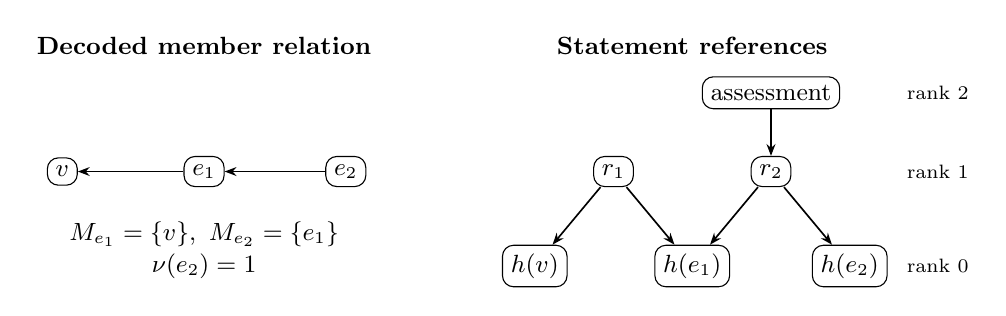
\begin{tikzpicture}[box/.style={draw,rounded corners,inner sep=3pt,font=\small},
ref/.style={-{Stealth[length=1.5mm]},semithick}]
\node[font=\small\bfseries] at (1.8,2.8) {Decoded member relation};
\node[box] (v) at (0,1.2) {$v$};
\node[box] (e1) at (1.8,1.2) {$e_1$};
\node[box] (e2) at (3.6,1.2) {$e_2$};
\draw[ref] (e2) -- (e1); \draw[ref] (e1) -- (v);
\node[font=\small] at (1.8,0.4) {$M_{e_1}=\{v\},\ M_{e_2}=\{e_1\}$};
\node[font=\small] at (1.8,0) {$\nu(e_2)=1$};
\node[font=\small\bfseries] at (8,2.8) {Statement references};
\node[box] (hv) at (6,0) {$h(v)$};
\node[box] (he1) at (8,0) {$h(e_1)$};
\node[box] (he2) at (10,0) {$h(e_2)$};
\node[box] (r1) at (7,1.2) {$r_1$};
\node[box] (r2) at (9,1.2) {$r_2$};
\node[box] (c) at (9,2.2) {assessment};
\draw[ref] (r1) -- (hv); \draw[ref] (r1) -- (he1);
\draw[ref] (r2) -- (he1); \draw[ref] (r2) -- (he2);
\draw[ref] (c) -- (r2);
\node[font=\scriptsize,anchor=west] at (10.6,0) {rank 0};
\node[font=\scriptsize,anchor=west] at (10.6,1.2) {rank 1};
\node[font=\scriptsize,anchor=west] at (10.6,2.2) {rank 2};
\end{tikzpicture}
\caption{Member roles $r_1=(h(e_1),\mg{member},h(v))$ and
$r_2=(h(e_2),\mg{member},h(e_1))$ encode nested edges at reference rank one. An optional
assessment of $r_2$ adds rank two, hence a third load stratum. The left arrows are decoded
member incidence; the right arrows are references between statement identifiers.}
\label{fig:depth}
\end{figure}

\begin{definition}[Compact binary encoding]
For an acyclic identified higher-order structure with singleton ends $y,z$, retain ground
Vertex anchors and encode each edge by one row $\kappa(h(e))=(h(y),p_e,h(z))$ with a fixed
node predicate $p_e$. Set $\delta(v)=0$ and $\delta(e)=1+\max(\delta(y),\delta(z))$.
\end{definition}
\begin{theorem}[Compact depth]\label{thm:compactrank}
$\rk(h(x))=\delta(x)$ for every atom in the compact encoding.
\end{theorem}
\begin{proof}
Induction on endpoint-dependency depth: vertices are ground anchors and each edge
references exactly its two encoded endpoints (one distinct referent if they agree).
\end{proof}
This restates the rank recurrence; its value is that, together with
Proposition~\ref{prop:strata}, it prices the compact encoding at $1+\delta_{\max}$ load
strata against two for the anchored one. Decoding compact stores needs a separate
convention to distinguish vertex anchors from edge rows, for example reserving
\iri{rdf:type} for anchors.
\begin{proposition}[Exact row counts]\label{prop:size}
Let $R=\sum_{e\in E}(|V_e|+|W_e|)$ and $U=\sum_{e\in E}|M_e|$. Directed and higher-order
encodings have $|X|+|E|+R$ rows; the member encoding has $|X|+|E|+U$ rows. For
Definition~\ref{def:annot}, with $Q=\sum_c|F_c|$ and $T=\sum_x|\mathrm{attr}(x)|$, the
encoding has $|A|+3|E\cup ME|+Q+T$ rows. Compact binary encoding has $|X|+|E|$ rows.
\end{proposition}
\begin{proof}
Count the disjoint anchor and field clauses of each encoding.
\end{proof}
These are row counts, not storage sizes: they ignore index and page overhead. With indexed
atom lookup and expected constant-time hash-set operations, encoding and decoding take
expected time linear in these counts. Not every image constraint is checkable row by row:
acyclicity needs traversal and extensionality needs comparison of grouped role sets.

\paragraph{Rank is not an epistemic type.}
A confidence row $(h(x),\iri{confidence},0.7)$ has rank one and a confidence on a
membership has rank two; both may express epistemic content. An approval represented as an
anchored event can have all structural rows at rank one, while an approval as a property of
a fact and an audit of that property give ranks one and two. Rank is an encoding-dependent
depth measure whose consumers are loading and retraction, not a test for reflection.

\section{A Provenance-Aware Memory Example}\label{sec:memory}
Episodic and semantic memory have distinct roles in cognitive accounts
\cite{tulving1972episodic}, and reconstruction and scripts motivate schema-guided recall
\cite{bartlett1932remembering,schank1977scripts}. Contemporary agent-memory systems
include temporal graph architectures and combined semantic/episodic world models
\cite{rasmussen2025zep,anokhin2024arigraph}. Our example concerns representation of their
kinds of information, not a comparison of retrieval performance.

\begin{example}[Membership with its own evidence]\label{ex:episode}
Let $a$ be a Vertex anchor marked as an episode container, $f$ a ground fact about Sarah's
job and $m$ its episode membership. The store contains:
\begin{center}\small
\begin{tabular}{lll}
\toprule
Identifier & Content & Rank\\
\midrule
$a$ & $(n_a,\iri{rdf:type},\mg{Vertex})$ & 0\\
$u$ & $(a,\mg{container},\mathit{true})$ & 1\\
$f$ & $(\iri{sarah},\iri{announced},\iri{newJob})$ & 0\\
$m$ & $(f,\sys{inGraph},a)$ & 1\\
$o$ & $(m,\iri{status},\iri{Observed})$ & 2\\
$c$ & $(m,\iri{confidence},0.7)$ & 2\\
$p$ & $(c,\iri{derivedFrom},\iri{transcript7})$ & 3\\
\bottomrule
\end{tabular}
\end{center}
A confidence $(f,\iri{confidence},0.9)$ about the job fact itself would have rank one, so
confidence in a fact and in its contextual membership are different claims. Loading this
store takes four strata (Proposition~\ref{prop:strata}); retracting $m$ removes $o$, $c$
and $p$ in at most two rounds (Proposition~\ref{prop:cascade}) and leaves $f$ and $a$. A
later dispute of $m$, valid in a year after $f$'s interval, is admissible under Policy~R of
Section~\ref{sec:time} and not under Policy~S. The store is an enriched $\NF4$
representation, not an exact attributed image.
\end{example}
Schemas can be marked containers whose slots are anchored atoms; slot fillings and
specialization are typed relations, and scripts add precedence relations between scene
anchors. These shapes do not enforce slot cardinality, satisfiability, causality or
temporal consistency of a script. An episode may contain observed, inferred, disputed or
recalled material, and membership alone does not imply observation; explicit status
predicates and derivation links record these distinctions. A constructive retrieval
procedure may emit default-based claims with \iri{Inferred} status linked to supporting
default occurrences, and retracting one default invalidates only a support depending on it;
we do not implement or evaluate it here. The six semantic categories proposed in
\cite{pavlyshyn2026metagraph} can be retained as type annotations; rank must not be used as
a substitute for them.

\section{Realization and Validation}\label{sec:evidence}
\subsection{Implementation boundary}
Tiramemsu is a Rust/SQLite statement-identity database with SPARQL and Cypher interfaces
\cite{pavlyshyn2026lbg}. Its repository recipe
\texttt{metagraph\_containers\_nesting\_and\_fold} demonstrates cyclic container
reachability, grouping without fact copying, an edge used as a graph name, and retraction
of memberships without deleting contained ground facts. One example query is:
\begin{verbatim}
PREFIX v: <urn:v:>
SELECT ?s WHERE {
  ?patient v:enrolledIn ?trial ~ ?edge .
  GRAPH ?edge { ?s ?p ?o }
}
\end{verbatim}
The statement-binding syntax is an engine extension. The engine does not enforce the image
constraints at write time and does not provide the metapath, dominance or projection
routines as library operators. The validators and checker below operate on finite stores
separately from engine execution.

\subsection{Executable validators}\label{sec:shacl}
The image constraints are expressible as executable validators over a row view of the
store: cardinality and class constraints as SHACL core shapes, and acyclicity
($\texttt{?e mg:member+ ?e}$) and extensionality (comparison of grouped role sets) as
SPARQL. The files, in \texttt{validators/}, are tested for agreement with the Python image
validators: on 80{,}665 store comparisons the SHACL and SPARQL verdicts and the Python
verdicts never differ. The comparisons are exhaustive for the roundtrip sources
under each family, for all 65{,}536 role-subset stores (2{,}401 accepted) and for the recursive
member sets, and sampled (seeded) for attributed stores and for single-row mutations of
valid stores. The row view projects each anchor row $(n,\iri{rdf:type},C)$ to a triple on
its identifier, because the toolchain used (rdflib, pyshacl) lacks RDF~1.2 reifier
patterns. This shows the images can be stated as shapes and queries over a standard
representation and that these agree with the checker on the tested sets; it does not make
the engine enforce them, and agreement on a finite set is not a proof.

\subsection{Reproduction protocol}\label{sec:checks}
The accompanying standard-library Python artifact, \texttt{check\_encodings.py} and
its extension module, retains source encoders, independently scanned image
validators and decoders, an incidence-search recognizer, an edge-sequence enumeration
oracle, a firing-closure implementation with a naive fixpoint oracle, and the property
tests listed below. Run:
\begin{verbatim}
python3 check_encodings.py --output validation-results.json
\end{verbatim}
\emph{Exhaustive enumeration} uses fixed bounds and no sampling. It covers directed and
higher-order roundtrips; all subsets of 16 possible role rows over two vertices and two
edges (including self-end roles); recursive member structures with cycle and
extensionality rejection; four-class attributed structures with empty and overlapping
fragments; metapath queries over all $B,C,F$ in a two-vertex, at-most-two-edge domain;
and the necessity witnesses of Table~\ref{tab:ablation}. Accepted candidate stores
equal the two-edge source encodings exactly: the 2{,}411 higher-order source roundtrips are
the 1 zero-edge, 9 one-edge and 2{,}401 two-edge sources, and the 2{,}401 accepted
candidates of Table~\ref{tab:validation} are that last group, seen from the store side.

\emph{Seeded randomized tests} (fixed seed, up to eight vertices and eight edges for
roundtrips and up to three edges for the sequence oracle) check, for each family,
roundtrip on random valid models; that any randomly mutated store the validator accepts
re-encodes to itself up to isomorphism; the strata and cascade propositions on random
$\NF4$ stores; firing closure against a naive fixpoint and Theorems~\ref{thm:exec}
and~\ref{thm:coincide} on random structures; and Theorem~\ref{thm:time} under both
policies on random histories. The oracle that enumerates edge sequences is exponential, so
its randomized domain is small. These tests exercise sizes beyond the exhaustive bounds
but remain finite samples, not proof.

\emph{Mechanized proof.} The directory \texttt{lean/} holds a Lean~4 development (core
library only) of the directed roundtrip, parametrized over $\Img{D}$, $\Img{HO}$ and the
extensional variants. It proves $\dec(\enc(M))\simeq M$ for valid sources,
$\enc(\dec(G))=G$ as row sets (and up to permutation) for image stores, membership of
$\enc(M)$ in the image, the row count of Proposition~\ref{prop:size}, and the rank bound of
Theorem~\ref{thm:flat} for these stores, with no \texttt{sorry}, axiom or
\texttt{native\_decide}. It fixes canonical identifiers, so it proves the clause
bijection of Lemma~\ref{lem:clause} rather than the quantification over renamings of
Definition~\ref{def:iso}; it models image membership as a scan-then-check predicate,
close to the validity of the decoded model, and it does not cover the recursive,
attributed or temporal results.

\begin{table}[t]
\centering\small
\begin{tabular}{L{10.2cm}r}
\toprule
Check family & Cases \\
\midrule
Exhaustive: directed roundtrips (identified edges) & 91 \\
Exhaustive: Basu--Blanning roundtrips (extensional) & 82 \\
Exhaustive: higher-order roundtrips ($1+9+2{,}401$ sources) & 2,411 \\
Exhaustive: higher-order candidate stores & 65,536 \\
Accepted / rejected candidates ($2{,}401$ = two-edge sources) & 2,401 / 63,135 \\
Exhaustive: recursive candidates / accepted roundtrips & 49 / 30 \\
Exhaustive: four-class attributed roundtrips & 65,536 \\
Exhaustive: metapath query/oracle comparisons & 5,488 \\
Exhaustive: compact depth configurations & 14,400 \\
Exhaustive: dependency-closed temporal selections & 20 \\
Targeted malformed-image rejections & 9 \\
Necessity witnesses (one per constraint) & 18 \\
Sampled: random valid models, roundtrip & 7,500 \\
Sampled: mutated stores accepted / rejected & 3,622 / 11,378 \\
Sampled: strata and cascade checks (random $\NF4$) & 1,500 \\
Exhaustive: firing-closure cases (3 vertices, $\le2$ edges) & 620,992 \\
Sampled: firing-closure cases with sequence oracle & 4,000 \\
Metapaths with coincidence antecedent / strict gap & 51,176 / 50,143 \\
Sampled: snapshot points, Policy R / Policy S & 24,000 / 24,000 \\
Sampled: version chains, violations rejected & 3,000 / 2,246 \\
\bottomrule
\end{tabular}

\caption{Counts produced by the retained checkers. A case is a model, store or query
configuration, not an independent theorem. Bounds and the exhaustive/sampled distinction
are recorded in \texttt{validation-results.json}.}
\label{tab:validation}
\end{table}
Passing finite checks supports the hand proofs and detects small counterexamples; it is not
proof for unbounded structures. The checker reports no performance measurements.

\section{Discussion and Limitations}\label{sec:discussion}
The practical consequence is a separation of concerns. A uniform carrier can retain
identity and annotate incidence, while the exact source image still needs explicit integrity
enforcement, and typed rows alone do not establish edge completeness, extensionality or
well-founded nesting. Row-level deletion and source-level deletion differ when one atom is
represented by several rows. Under time, extensional images are fragile
(Remark~\ref{rem:fragile}), which favours the identified images.

\paragraph{Scope.}
The source restrictions matter: directed ends and recursive edges are nonempty, recursive
incidence is well founded and attributed values are ground. Annotating presentations
that identify atoms by all their fields, allow other endpoint classes or attach
graph-valued attributes need different signatures and images. We do not claim that
identified triples are a minimal universal storage primitive, that inclusion of row
languages is a semantic expressiveness separation, that these encodings are faster,
smaller or more expressive than relational or graph alternatives, or that reference
rank classifies epistemic content. A systems evaluation should compare matched incidence
and reification baselines \cite{hernandez2015reifying}, include index and storage overhead
and separate role-heavy reads from integrity-maintaining updates; a memory-system
evaluation should measure retrieval and provenance handling with ablations of identity,
annotated membership and time. Neither is part of this paper.

\paragraph{Evidence.}
Validation is finite enumeration, seeded randomized testing, executable validators and a
partial Lean proof; there is no external review. The mechanized proof covers one family under
canonical naming. Version propagation under revision, effective validity on read and the
general dominant-metapath problem are not treated. Full-text comparison with the three
recent metagraph works remains necessary before any priority claim about operations or
granulation. The accompanying source audit records access limits and the reference
metadata checked in this revision; the inherited bibliography has not been wholly audited.

\section{Conclusion}
Identified triples admit invertible encodings of explicitly specified finite metagraph
structures when exact image constraints distinguish identity, incidence and containment,
and each constraint is necessary. Under time, a policy that retains referents of asserted
rows lets annotations live outside their bearer's interval, and a supersession relation
records identity across versions. Executable metapaths can be recognized in linear
incidence size and coincide with walk metapaths when the dependency graph is acyclic or
tails are singletons. Reference rank prices loading and retraction. Enforcing these
contracts efficiently in an engine and measuring their value for agent memory remain
implementation and evaluation tasks.

\paragraph{Availability.}
The source, PDF, checkers, validators, Lean proof and validation results accompany
Tiramemsu at \url{https://github.com/Volland/tiramemsu}, in
\path{paper/metagraphs-from-identified-triples/}. Tiramemsu uses MIT and Apache-2.0 licenses.
\bibliographystyle{plainnat}
\bibliography{references}
\end{document}
